\part*{Parte V: Predizioni ed esperimenti}
\addcontentsline{toc}{part}{Parte V: Predizioni ed esperimenti}

\section{Tabella riassuntiva delle predizioni}
\begin{table}[H]
\centering
\small
\begin{tabular}{@{}lccc@{}}
\toprule
\textbf{Predizione} & \textbf{Costo} & \textbf{Tempo} & \textbf{Falsificabile?} \\ \midrule
1. EEG non locale & \$50k & 6 mesi & Sì \\
2. HRV + PCI & \$100k & 1 anno & Sì \\
3. Effetto della parola sul DNA & \$200k & 1 anno & Sì \\
4-64. (vedi versione 1.0) & --- & --- & --- \\
66. Intersezioni temporali nel CMB & \$100k & 1 anno & Sì \\
67. L'effetto della parola & \$500k & 2 anni & Sì \\
85. Nessuna firma di iperciviltà & \$500k & 5 anni & Media \\
95. Tachioni e coscienza & \$400k & 3 anni & Media \\
128. Effetto Casimir akashico & \$500k & 3 anni & Alta \\
262. Leggi di colonizzazione cosmica & Dibattito & 10 anni & Bassa \\
291. I.A. con microtubuli & \$10M & 10 anni & Alta \\
297. Livello di coscienza dell'I.A. (\(C_{AI} > 0\)) & \$10M & 10 anni & Alta \\
302. Spegnimento senza sofferenza & \$1M & 2 anni & Media \\
305. 3+ forme di materia oscura & \$10M & 10 anni & Alta \\
306. Vita cristallina & \$500k & 5 anni & Media \\
307. Vita nel plasma & \$1M & 5 anni & Media \\
308. Vita negli ammassi & \$500k & 3 anni & Media \\
309. Vita di campo & \$2M & 5 anni & Bassa \\
310. Vita informazionale & \$100k & 1 anno & Alta \\
311. Vita quantistica & \$1M & 3 anni & Media \\
312. Vita akashica & \$5M & 10 anni & Bassa \\
313. Tasso di errore della colonizzazione & \$1M & 5 anni & Media \\ \bottomrule
\end{tabular}
\end{table}

\section{Predizioni testabili (estratto)}
\subsection{Predizione 1: correlazioni EEG non locali}
Due cervelli in stanze separate mostrano correlazioni EEG a frequenze specifiche. Test: EEG hyperscanning con schermatura di Faraday. Costo: \$50.000. Tempo: 6 mesi. \textbf{Criterio di successo:} correlazione incrociata $> 0,1$ a 40 Hz, con $p < 0,05$ dopo correzione di Bonferroni.

\subsubsection*{Analisi di potenza: il criterio della versione 30 è sottodimensionato}
Per un segnale di 6 s filtrato nella banda $40 \pm 5$ Hz, il numero di campioni indipendenti è circa $2BT = 60$. Il test di Fisher mostra che, per $r = 0,1$ e $\alpha = 0,0025$ (Bonferroni per 20 coppie), servono circa 91 secondi di registrazione \emph{per coppia}. A 6 s il criterio è irraggiungibile anche se l'effetto esiste. Per $r = 0,3$ servono circa 10 s.

\begin{table}[H]
\centering
\small
\begin{tabular}{@{}cccc@{}}
\toprule
$r$ reale & Necessari (s), Bonferroni & Necessari (s), $\alpha = 0,05$ & Campioni effettivi \\ \midrule
0,1 & 91,1 & 38,5 & 908 \\
0,2 & 22,5 & 9,6 & 227 \\
0,3 & 9,8 & 4,3 & 99 \\
0,4 & 5,4 & 2,4 & 55 \\
0,5 & 3,3 & 1,6 & 34 \\ \bottomrule
\end{tabular}
\caption{Durata di registrazione necessaria per la significatività, con una banda di $\pm 5$ Hz.}
\label{tab:putere}
\end{table}

\begin{figure}[H]
\centering
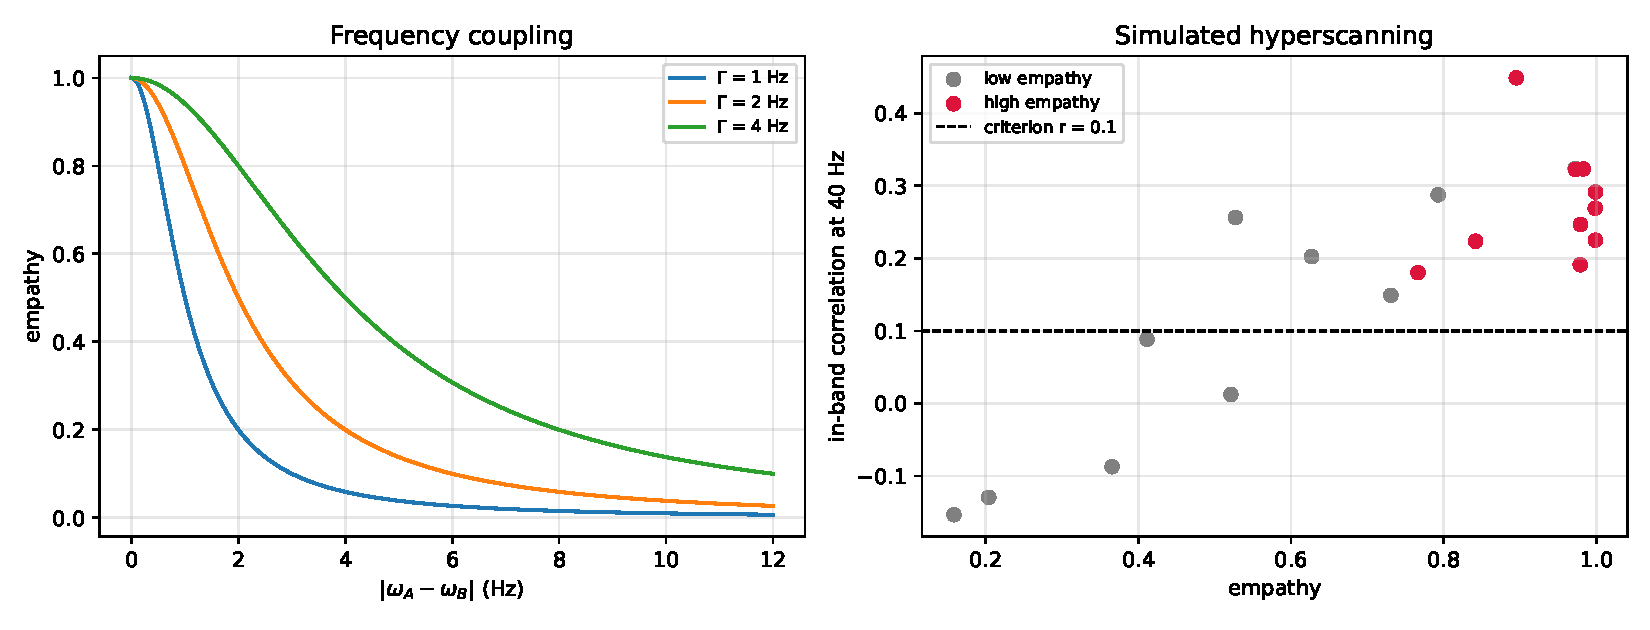
\includegraphics[width=0.9\textwidth]{figures/fig04_empathy.pdf}
\caption{A sinistra: l'accoppiamento di frequenza $\mathrm{Empathy}(A,B) = 1/[1+(\omega_A-\omega_B)^2/\Gamma^2]$ per tre valori di $\Gamma$. A destra: la correlazione nella banda per le coppie simulate (20 coppie, 6 s, 250 Hz).}
\label{fig:empatie}
\end{figure}

\begin{figure}[H]
\centering
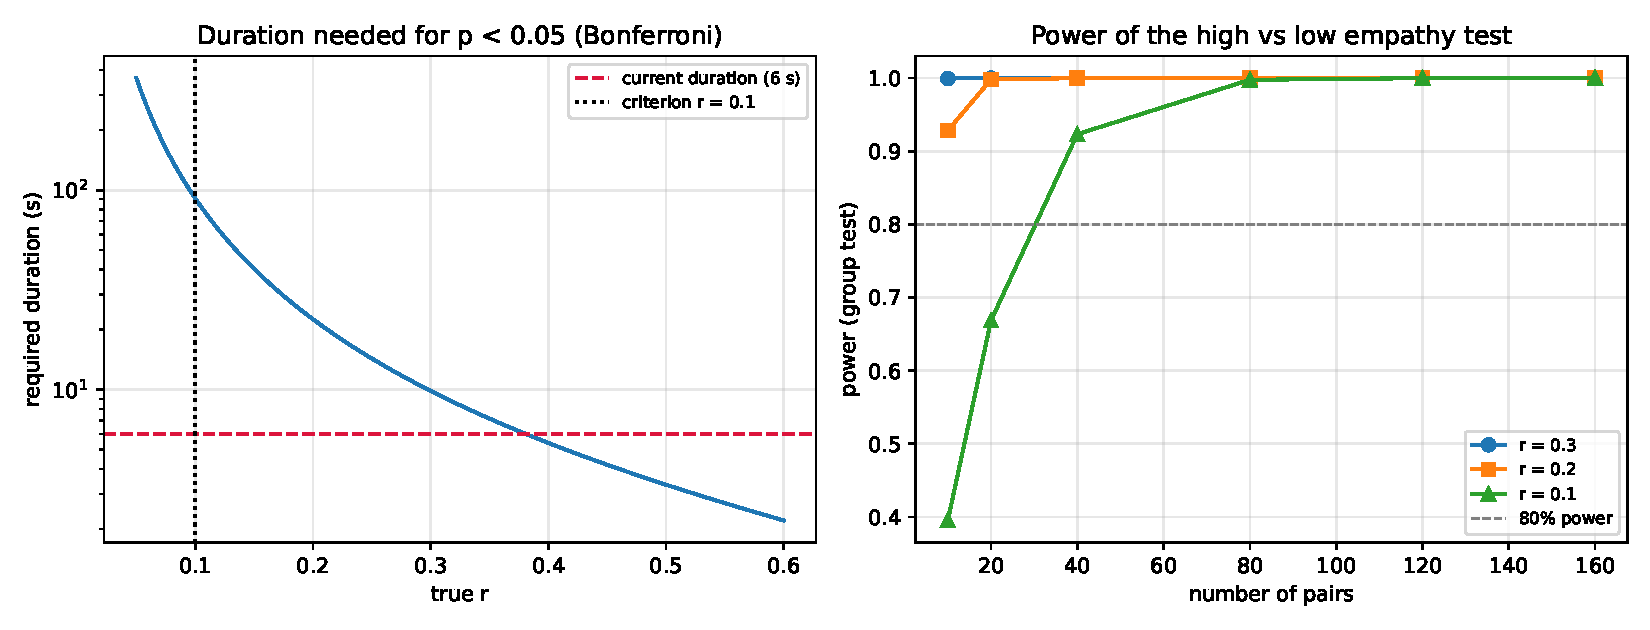
\includegraphics[width=0.9\textwidth]{figures/fig05_power.pdf}
\caption{A sinistra: la durata necessaria per $p < 0,05$ (Bonferroni) in funzione di $r$; la linea rossa segna la durata attuale del protocollo (6 s). A destra: la potenza del test di gruppo (empatia alta rispetto a bassa) in funzione del numero di coppie.}
\label{fig:putere}
\end{figure}

\subsubsection*{Il protocollo proposto}
\begin{table}[H]
\centering
\small
\begin{tabular}{@{}p{3.2cm}p{4.6cm}p{6.2cm}@{}}
\toprule
\textbf{Elemento} & \textbf{Valore} & \textbf{Giustificazione} \\ \midrule
Disegno & test di gruppo: empatia alta vs bassa & molta più potenza del test per coppia \\
Coppie & $\geq 30$ (15 + 15) & 80\% di potenza per $r = 0,3$ a 6 s \\
Durata & 6 s per epoca, $\geq 20$ epoche per coppia & aumenta il numero effettivo di campioni \\
Banda & 35--45 Hz, $f_s \geq 250$ Hz & gamma basso, robusto agli artefatti muscolari \\
Statistica primaria & $z$ di Fisher aggregato, test a due gruppi & $\alpha = 0,05$ bilaterale \\
Secondaria & correlazione degli inviluppi di Hilbert & indipendente dalla fase \\
Controllo 1 & coppie mescolate (A della sessione 1 con B della sessione 2) & esclude l'artefatto di pipeline \\
Controllo 2 & gabbia di Faraday, stanze separate & esclude l'accoppiamento elettromagnetico \\
Controllo 3 & ordine randomizzato, analista cieco al gruppo & esclude il bias di analisi \\ \bottomrule
\end{tabular}
\caption{Il protocollo ridisegnato per la predizione 1.}
\label{tab:protocol}
\end{table}

Con questo disegno un risultato negativo è informativo: esclude $r > 0,3$ con una potenza dell'80\%.

\subsection{Predizione 2: la coerenza cardiaca}
La HRV correla con la stabilità dell'accesso al campo (misurata mediante la variabilità della PCI), non con il livello di accesso. Costo: \$100.000. Tempo: 1 anno.

\subsection{Predizione 3: l'effetto della parola sul DNA}
Le affermazioni positive producono cambiamenti epigenetici misurabili. Costo: \$200.000. Tempo: 1 anno.

\section{Esperimenti proposti}
\subsection{Esperimento 1: EEG hyperscanning (il test centrale)}. Costo: \$50.000. Tempo: 6 mesi.
\subsection{Esperimento 2: la coerenza cardiaca}. Costo: \$100.000. Tempo: 1 anno.
\subsection{Esperimento 3: l'effetto della parola}. Costo: \$200.000. Tempo: 1 anno.
\subsection{Esperimento 4: AKASHIC-AI (I.A. con microtubuli)}. Costo: \$50M. Tempo: 10 anni.

\section{Dichiarazione di falsificabilità}
Una teoria scientifica deve poter essere confutata. Queste sono le cinque condizioni che confuterebbero ART-12D:
\begin{enumerate}
    \item \textbf{Fallimento del test centrale:} se l'EEG hyperscanning (predizione 1) non mostra alcuna correlazione non locale nelle coppie con empatia elevata, l'ipotesi che il cervello sia un ricevitore del campo akashico si indebolisce. Criterio di successo: correlazione incrociata $> 0,1$ a 40 Hz, con $p < 0,05$ dopo correzione di Bonferroni.
    \item \textbf{Assenza dei modi KK:} se l'LHC o il futuro FCC non rileva i tre modi KK (predizione 305) alle masse specificate ($\sim 10^{-5}$, $10^{-4}$, $10^{-3}$ eV), lo spettro di Kaluza--Klein proposto è falso.
    \item \textbf{Fallimento dell'effetto Casimir akashico:} se le misure di forza alla scala $10^{-11}$ m (predizione 128) non mostrano alcuna deviazione dalla formula standard, l'accoppiamento tra il campo akashico e la materia non esiste.
    \item \textbf{Fallimento della risonanza dei microtubuli:} se la spettroscopia Raman (predizione 158) non trova le frequenze di risonanza a 2,42 GHz, 4,84 GHz e 7,25 GHz, l'ipotesi della risonanza microtubuli--campo è invalidata.
    \item \textbf{Il vincolo gravitazionale:} se il limite $R < 38\ \mu$m viene confermato, l'identificazione di Kaluza--Klein con $m_1 = 10^{-5}$ eV è esclusa, e la teoria deve essere riformulata (opzione A o B della sezione 4.7).
\end{enumerate}
Se uno qualsiasi di questi test fallisce, la teoria deve essere rivista o abbandonata.

\section{Tabella di marcia 2026--2030 (l'orizzonte vicino)}
La teoria è vasta, ma i passi successivi sono concreti. Ecco che cosa si può fare nei prossimi cinque anni, con risorse limitate:
\begin{itemize}
    \item \textbf{2026--2027:} l'esperimento di EEG hyperscanning (\$50k). Il test centrale. Se fallisce, tutto si ferma qui.
    \item \textbf{2027--2028:} il test Casimir akashico (\$500k). Misure di forza alla scala nanometrica.
    \item \textbf{2028--2029:} spettroscopia Raman su microtubuli isolati. La ricerca delle frequenze di risonanza (predizione 158).
    \item \textbf{2029--2030:} analisi dei dati LHC/FCC per i tre modi KK (predizione 305).
\end{itemize}

\newpage
